\documentclass[compress]{beamer}
\usepackage{ifthen,verbatim}

\newcommand{\isnote}{}
\xdefinecolor{lightyellow}{rgb}{1.,1.,0.25}
\xdefinecolor{darkblue}{rgb}{0.1,0.1,0.7}

%% Uncomment this to get annotations
%% \def\notes{\addtocounter{page}{-1}
%%            \renewcommand{\isnote}{*}
%% 	   \beamertemplateshadingbackground{lightyellow}{white}
%%            \begin{frame}
%%            \frametitle{Notes for the previous page (page \insertpagenumber)}
%%            \itemize}
%% \def\endnotes{\enditemize
%% 	      \end{frame}
%%               \beamertemplateshadingbackground{white}{white}
%%               \renewcommand{\isnote}{}}

%% Uncomment this to not get annotations
\def\notes{\comment}
\def\endnotes{\endcomment}

\setbeamertemplate{navigation symbols}{}
\setbeamertemplate{headline}{\mbox{ } \hfill
\begin{minipage}{5.5 cm}
\vspace{-0.75 cm} \small
\end{minipage} \hfill
\begin{minipage}{4.5 cm}
\vspace{-0.75 cm} \small
\begin{flushright}
\ifthenelse{\equal{\insertpagenumber}{1}}{}{Jim Pivarski \hspace{0.2 cm} \insertpagenumber\isnote/\pageref{numpages}}
\end{flushright}
\end{minipage}\mbox{\hspace{0.2 cm}} \hspace{0.01 cm} \vspace{-1.05 cm}}

\newcommand{\s}[1]{{\mbox{\scriptsize #1}}}

\begin{document}
\begin{frame}
\vfill
\begin{center}
\textcolor{darkblue}{\Huge Spin!}

\vfill
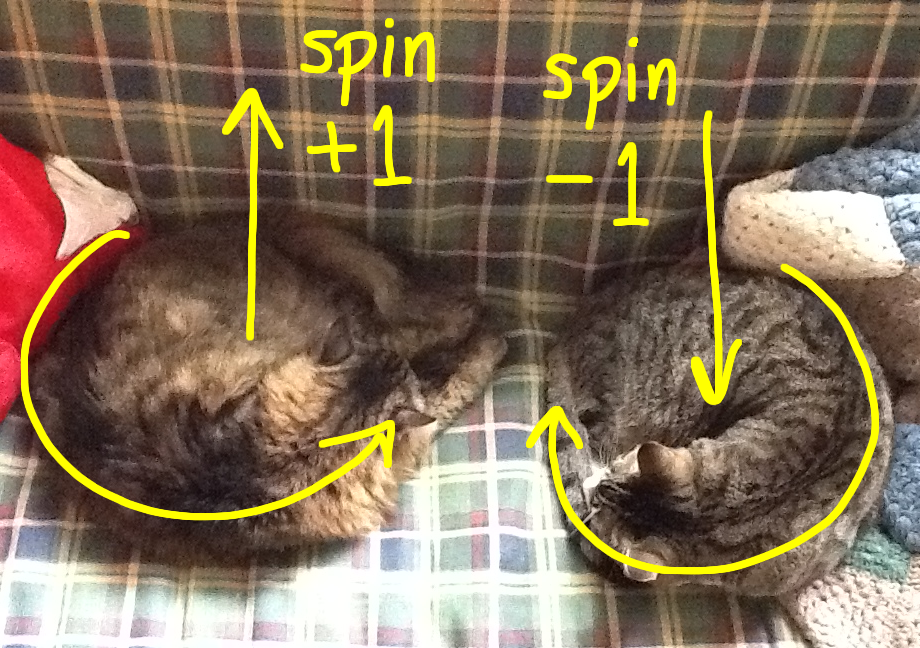
\includegraphics[width=0.5\linewidth]{spin-0.png}

\vfill
\begin{columns}
\column{0.3\linewidth}
\begin{center}
\large
Jim Pivarski
\end{center}
\end{columns}

%% \begin{columns}
%% \column{0.3\linewidth}
%% \begin{center}
%% \scriptsize
%% {\it Fermilab}
%% \end{center}
%% \end{columns}

\vfill
17 November, 2012

\end{center}
\end{frame}

%% \begin{notes}
%% \item This is the annotated version of my talk.
%% \item If you want the version that I am presenting, download the one
%% labeled ``slides'' on Indico (or just ignore these yellow pages).
%% \item The annotated version is provided for extra detail and a written
%% record of comments that I intend to make orally.
%% \item Yellow notes refer to the content on the {\it previous} page.
%% \item All other slides are identical for the two versions.
%% \end{notes}

\small

\begin{frame}
\frametitle{Betting on the Higgs discovery (June 17)}
\vfill
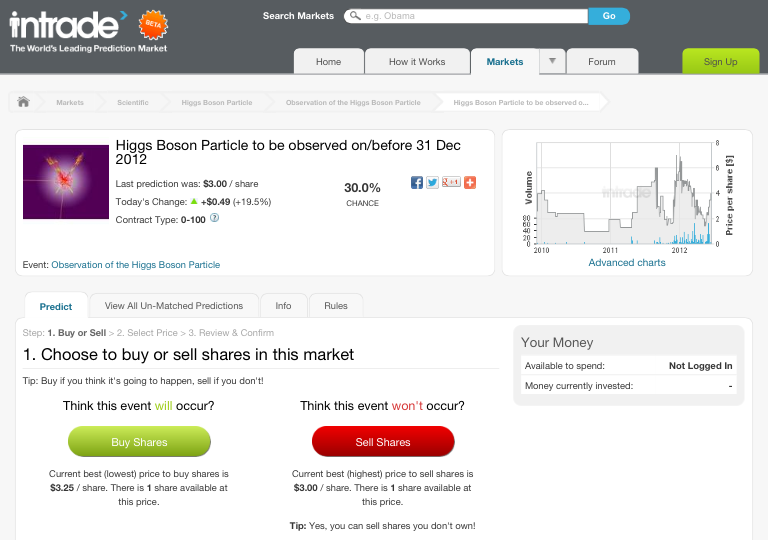
\includegraphics[width=\linewidth]{higgs_trading.png}
\end{frame}

\begin{frame}
\frametitle{Betting on the Higgs discovery (June 17)}
\vfill
The rules were careful about some issues (peer reviewed journal, independent confirmation, five sigma statistical significance)\ldots
\vfill
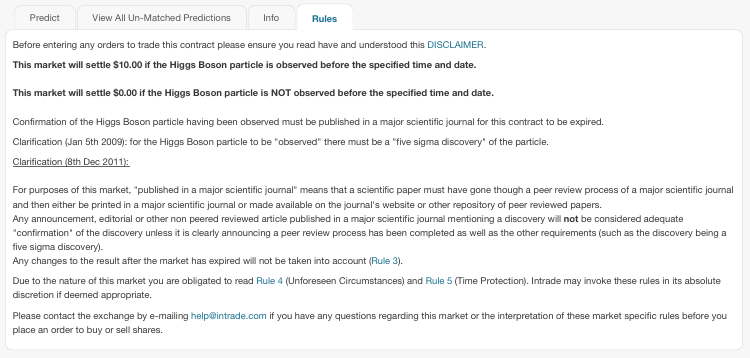
\includegraphics[width=\linewidth]{doesnt_mention_spin.png}
\vfill
\textcolor{blue}{But they didn't actually require the new particle to be a Higgs boson.}
\vfill
The market closed on Sep 11, 2012 (the publication date of the discovery), but we still don't know if a Higgs was discovered.
\end{frame}

\begin{frame}
\frametitle{What is a Higgs?}

Some essential properties (to solve the problem for which it was intended):
\begin{itemize}
\item Non-zero vacuum expectation value
\item Couples to particles in proportion to their masses
\item Spin-0
\end{itemize}

Some non-essential properties (variants of the basic theory):
\begin{itemize}
\item Fermiophobic (only explains boson masses, not fermion masses)
\item Supersymmetric (fits into a larger context that explains the Higg's own mass)
\item Two-doublet (multiple Higgses, each bearing a part of the load)
\item Metastable (the evacuum expectation value might change)
\end{itemize}
\end{frame}

\begin{frame}
\frametitle{What is a Higgs?}

\textcolor{gray}{Some essential properties (to solve the problem for which it was intended):}
\begin{itemize}
\item \textcolor{gray}{Non-zero vacuum expectation value}
\item \textcolor{gray}{Couples to particles in proportion to their masses}
\item \textcolor{red}{Spin-0}
\end{itemize}

\textcolor{gray}{Some non-essential properties (variants of the basic theory):}
\begin{itemize}
\item \textcolor{gray}{Fermiophobic (only explains boson masses, not fermion masses)}
\item \textcolor{gray}{Supersymmetric (fits into a larger context that explains the Higg's own mass)}
\item \textcolor{gray}{Two-doublet (multiple Higgses, each bearing a part of the load)}
\item \textcolor{gray}{Metastable (the evacuum expectation value might change)}
\end{itemize}
\end{frame}

\begin{frame}
\frametitle{This talk is about spin}
\begin{center}
\begin{minipage}{0.8\linewidth}
\begin{itemize}\setlength{\itemsep}{0.5 cm}
\item Classical angular momentum
\item Spin: angular momentum in quantum mechanics
\item Examples of quantized spin, some visible to the naked eye
\item Measuring the new particle's spin
\end{itemize}
\end{minipage}
\end{center}
\end{frame}

\begin{frame}
\frametitle{Angular momentum}
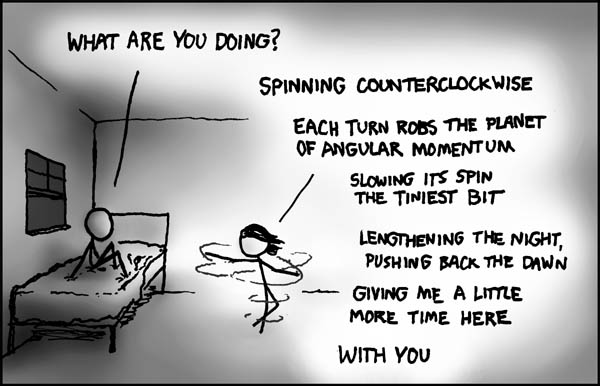
\includegraphics[width=\linewidth]{angular_momentum.jpg}

\hfill \textcolor{blue}{\scriptsize \url{http://xkcd.com/}}
\end{frame}

\begin{frame}
\frametitle{Angular momentum}
\begin{center}
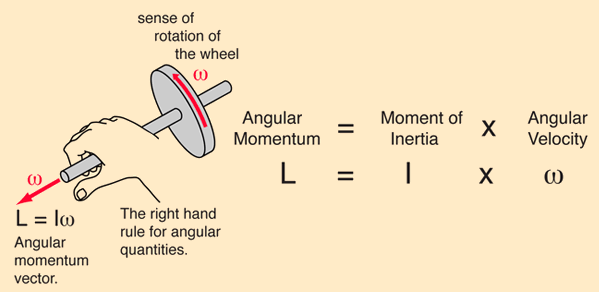
\includegraphics[width=0.6\linewidth]{angular_momentum.png}
\end{center}

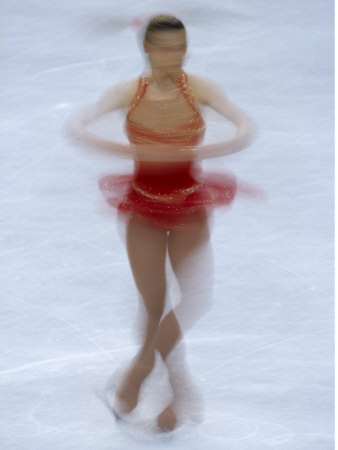
\includegraphics[height=3 cm]{spinning_skater.jpg} \hfill
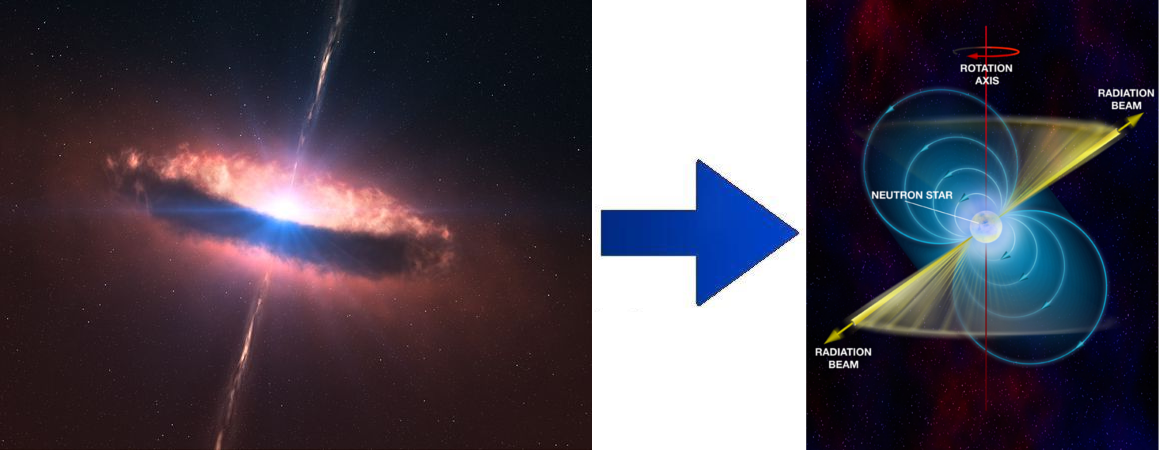
\includegraphics[height=3 cm]{accretion_disk_to_pulsar.png}
\end{frame}

\begin{frame}
\frametitle{Quantized angular momentum}

Angular momentum $\vec{L} = \vec{r} \times \vec{p}$ = position times momentum.

\vspace{0.2 cm}
Position times momentum is quantized in units of

\hfill $\hbar/2 = 5.27 \times 10^{-35}$ meter $\cdot$ Newton-seconds.

\begin{columns}
\column{0.3\linewidth}
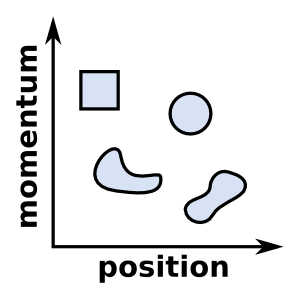
\includegraphics[width=\linewidth]{equal_area.png}
\column{0.7\linewidth}

Phase space (momentum vs.\ position) is granular at an extremely small scale.

\vspace{0.3 cm}
Related to $\Delta x \Delta p \ge \hbar/2$.

\end{columns}

\vfill
The angular momentum of an individual particle is only one or two units, called spin.
\end{frame}

\begin{frame}
\frametitle{Spin of fundamental particles}

\vspace{-0.6 cm}
\begin{tabular}{p{0.2\linewidth} p{0.2\linewidth} p{0.2\linewidth} p{0.2\linewidth}}
\begin{center} spin-0 \end{center} & \begin{center} spin-$\frac{1}{2}$ ($\hbar/2$) \end{center} & \begin{center} spin-1 ($\hbar$) \end{center} & \begin{center} spin-2 ($2\hbar$) \end{center} \\
Higgs bosons & Quarks, electrons, muons, taus, neutrinos & Photons, \mbox{W, Z} bosons, gluons & \mbox{ } \hfill Gravitons \hfill \mbox{ } \\
\end{tabular}

\vspace{0.2 cm}
Angular momentum of composite particles, such as protons (3 quarks), is the sum of these ``intrinsic'' spins and physical rotation.

\vfill
\hspace{-0.83 cm} \uncover<2->{\textcolor{darkblue}{\Large Photon spin is circular polarization}}

\vspace{0.2 cm}
\uncover<2->{All photons have total spin 1; some in the direction of travel ($+1$), some opposite to the direction of travel ($-1$).  Used to project 3-D movies.}

\uncover<2->{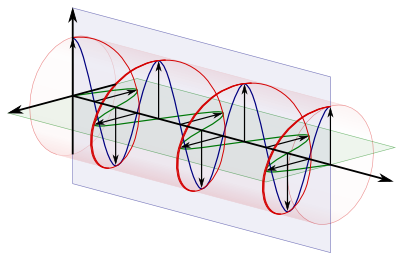
\includegraphics[height=2.5 cm]{polarized_wave.png} \hfill 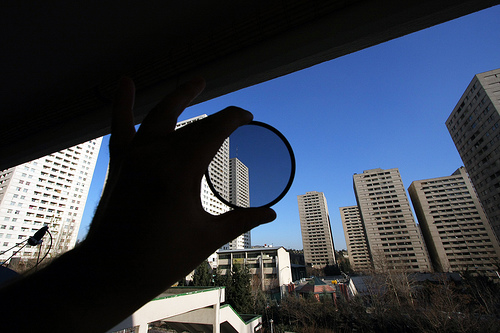
\includegraphics[height=2 cm]{polarized_filter.jpg} \hfill 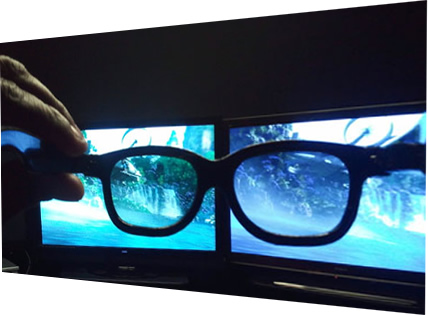
\includegraphics[height=2 cm]{three-d_glasses.jpg}}
\end{frame}

\setbeamertemplate{headline}{\mbox{ } \hfill
\begin{minipage}{5.5 cm}
\vspace{-0.75 cm} \small
\end{minipage} \hfill
\begin{minipage}{4.5 cm}
\vspace{-0.75 cm} \small
\begin{flushright}
\ifthenelse{\equal{\insertpagenumber}{1}}{}{\hspace{0.2 cm} \insertpagenumber\isnote/\pageref{numpages}}
\end{flushright}
\end{minipage}\mbox{\hspace{0.2 cm}} \hspace{0.01 cm} \vspace{-1.05 cm}}

\begin{frame}
\frametitle{Quantized angular momentum, big enough to see}

I have a problem with the idea that something related to rotation is quantized.  Why not just put it on a record player and turn it slowly?

\vfill
\begin{columns}
\column{0.25\linewidth}

This experiment was performed with liquid helium, a quantum system big enough to see.

\vspace{0.2 cm}
The result: \mbox{quantized vortices} emerged to cancel the angular momentum.

\vspace{0.5 cm}
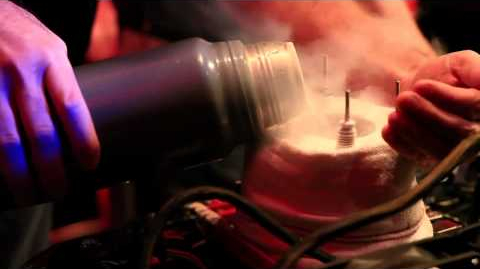
\includegraphics[width=\linewidth]{liquid_helium_pouring.jpg}

\column{0.65\linewidth}
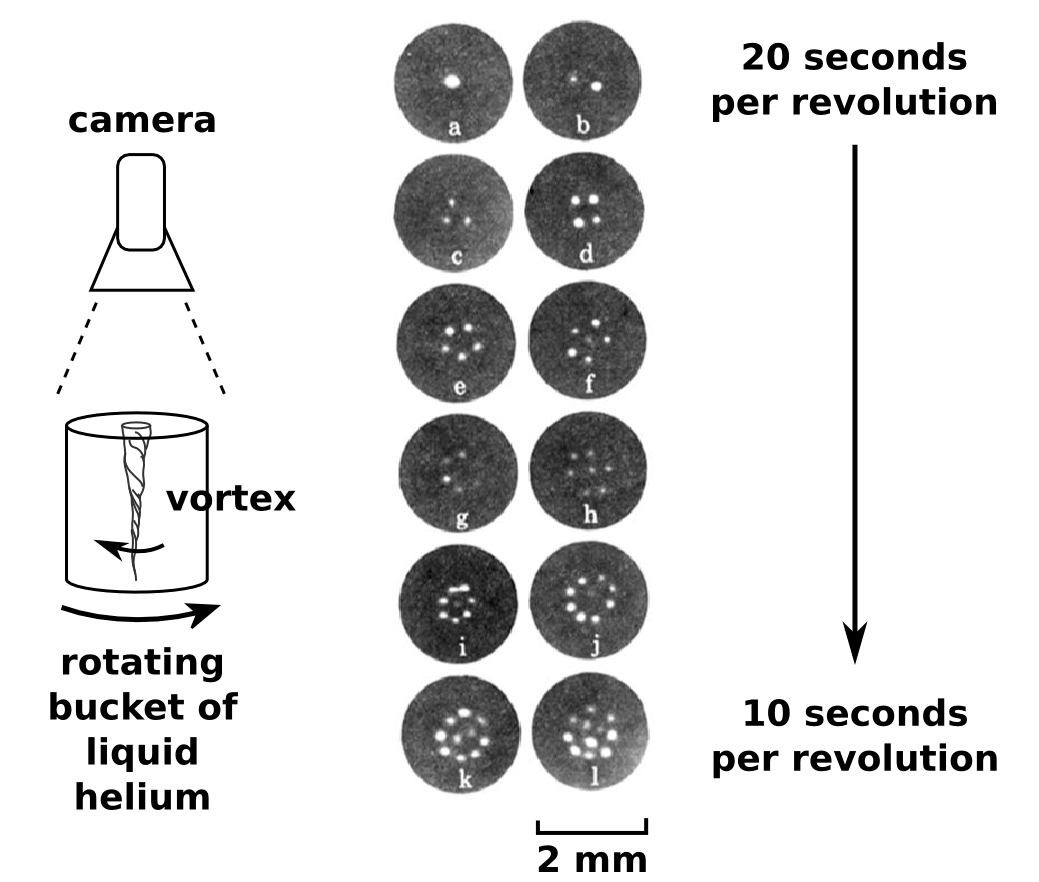
\includegraphics[width=\linewidth]{quantized_vortices.png}
\end{columns}
\end{frame}

\setbeamertemplate{headline}{\mbox{ } \hfill
\begin{minipage}{5.5 cm}
\vspace{-0.75 cm} \small
\end{minipage} \hfill
\begin{minipage}{4.5 cm}
\vspace{-0.75 cm} \small
\begin{flushright}
\ifthenelse{\equal{\insertpagenumber}{1}}{}{Jim Pivarski \hspace{0.2 cm} \insertpagenumber\isnote/\pageref{numpages}}
\end{flushright}
\end{minipage}\mbox{\hspace{0.2 cm}} \hspace{0.01 cm} \vspace{-1.05 cm}}

\begin{frame}
\frametitle{Why the Higgs must have no spin}

A little more background about the Higgs mechanism:
\begin{itemize}
\item All particles are excitations of fields: the quark field, the electron field, the photon field ($\vec{E}$ and $\vec{B}$), etc.
\item The vacuum is the minimum energy state.  For most fields, this means the field value is zero (e.g.\ $\vec{E}=0$, $\vec{B}=0$ means no photons).
\item The Higgs field has a minimum energy state that is not zero; everywhere in the universe, the Higgs field is present, to interact with particles and give them the illusion of having mass.
\item A Higgs particle is an excitation around that non-zero minimum.
\end{itemize}

The vacuum does not have a preferred direction in space: it is rotationally symmetric.  Fields with spin are asymmetric when they are non-zero because angular momentum is a vector.

\vfill
The Higgs field must be non-zero everywhere and {\it not} rotationally asymmetric.  Hence it must have no spin.

\end{frame}

\begin{frame}
\frametitle{What do we know about the new particle?}

\begin{columns}
\column{0.4\linewidth}
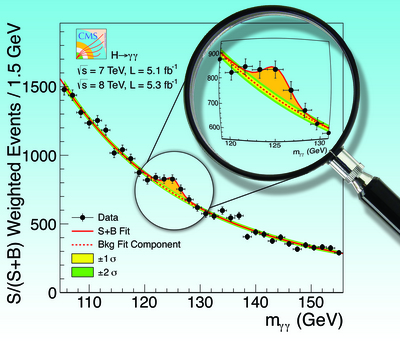
\includegraphics[width=\linewidth]{new_boson_125_small.jpg}

\vspace{0.2 cm}
\begin{minipage}{\linewidth}
\scriptsize (Only showing CMS results: adding results from other experiments increases confidence.)
\end{minipage}

\column{0.6\linewidth}
Something with mass = 126~GeV decays to
\begin{itemize}
\item two photons (99.9937\% confidence)
\item two Z bosons (99.9989\% confidence)
\end{itemize}
Something with a mass in the 120--130~GeV ballpark decays to
\begin{itemize}
\item two W bosons (99.73\% confidence)
\item two b quarks (92.8\% ``hint'')
\item two taus (92.8\% ``hint'')
\end{itemize}
\end{columns}

\vfill
Only spin-0 and spin-2 particles can decay into two photons (the most restrictive decay mode).
\end{frame}

\begin{frame}
\frametitle{Angular momentum conserved in decays}

A spin-0 particle can decay into two photons with oppositely aligned spins: $0 = (+1) + (-1)$.

\vfill
A spin-2 particle can decay into two photons with the same spin: $(+2) = (+1) + (+1)$\hspace{0.5 cm}or\hspace{0.5 cm}$(-2) = (-1) + (-1)$.

\vfill
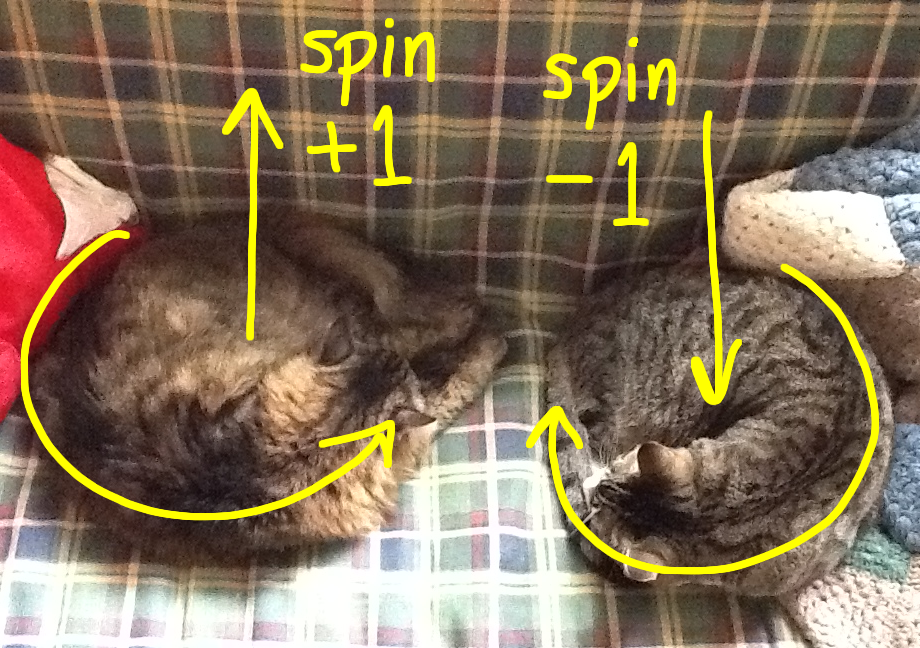
\includegraphics[height=3.4 cm]{spin-0.png} \hfill 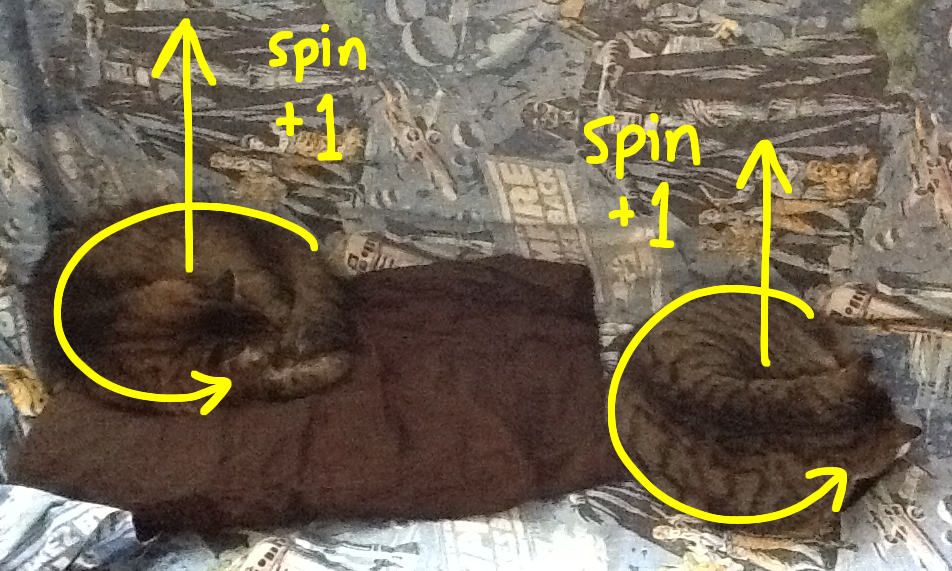
\includegraphics[height=3.4 cm]{spin-2.png}

\vfill
{\it However,} we can't easily measure the spin of these photons.  Their energy is 30 billion times too high for photographic filters.
\end{frame}

\begin{frame}
\frametitle{Measuring spin from decay angles}

When particles decay, the angle of the decay products is random, but with a probability distribution that depends on spin.

\vfill
\begin{columns}
\column{0.32\linewidth}
\centering spin-0

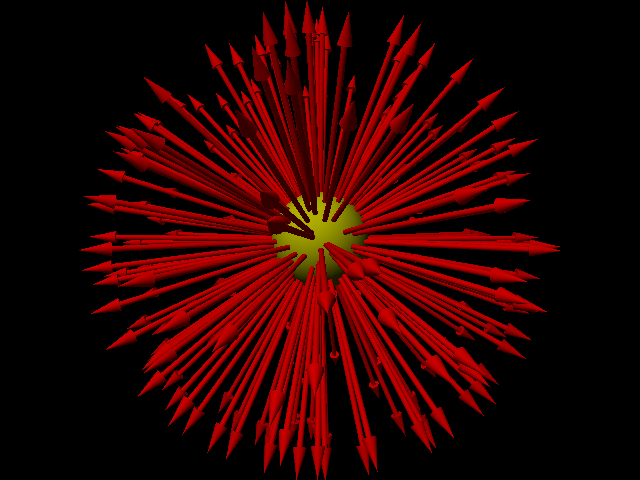
\includegraphics[width=\linewidth]{spin0.png}

\column{0.32\linewidth}
\centering spin-1

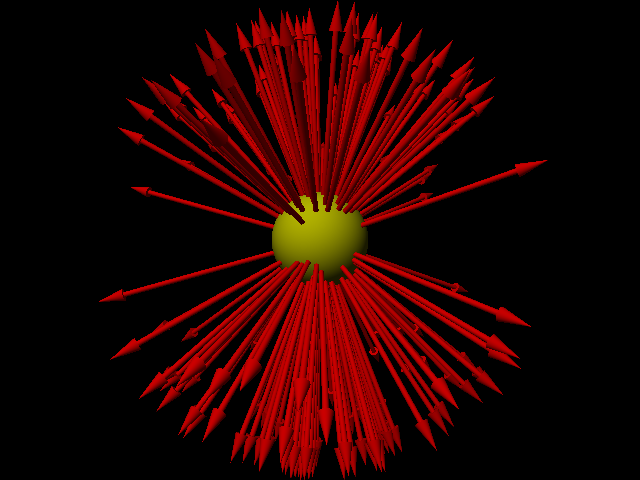
\includegraphics[width=\linewidth]{spin1.png}

\column{0.32\linewidth}
\centering spin-2

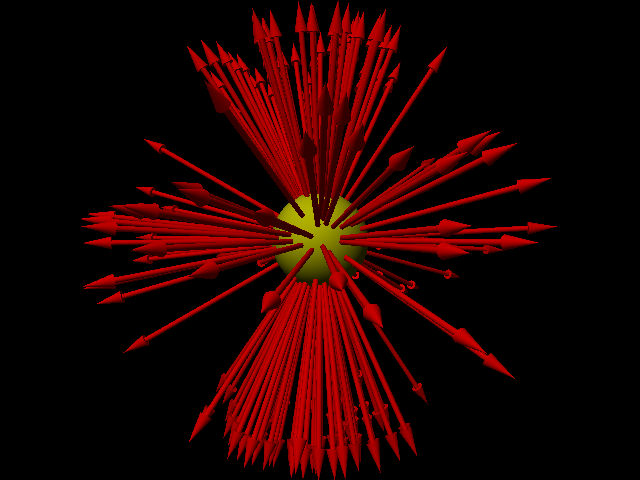
\includegraphics[width=\linewidth]{spin2.png}
\end{columns}

\vfill
Spin-0 particles have no preferred direction in space, so a large sample of spin-0 particles decay symmetrically.

\vfill
Spin-1 particles prefer to decay toward or against their angular momentum vector.

\vfill
Spin-2 particles have a more complicated pattern: toward the poles or along the equator.
\end{frame}

\begin{frame}
\frametitle{Measuring spin from decay angles}

The Higgs to ZZ decay has the most experimental ``handles,'' since Z bosons are spin-1 objects that decay into muons, which have very distinctive tracks.  The analysis gets complicated, though:
\begin{center}
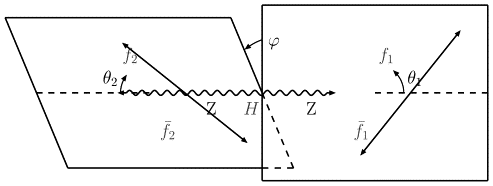
\includegraphics[width=0.5\linewidth]{HZZspins.png}
\end{center}

\vfill
\begin{columns}
\column{0.5\linewidth}
Another option is to produce Higgses in electron collisions, which is like a Higgs decay to electrons in reverse.

\vspace{0.2 cm}
The Higgs production rate versus electron energy depends on spin.

\column{0.35\linewidth}
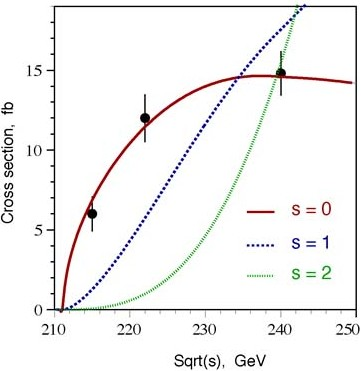
\includegraphics[width=\linewidth]{ILCspin.jpg}
\end{columns}
\end{frame}

%% \begin{frame}
%% \frametitle{Outline}
%% \begin{itemize}\setlength{\itemsep}{0.75 cm}
%% \item 
%% \end{itemize}
%% %% \hspace{-0.83 cm} \textcolor{darkblue}{\Large Outline2}
%% \end{frame}

%% \section*{First section}
%% \begin{frame}
%% \begin{center}
%% \Huge \textcolor{blue}{First section}
%% \end{center}
%% \end{frame}

\begin{frame}
\frametitle{The bottom line}

We don't have enough events to determine the spin of the new particle!
\begin{itemize}
\item Many events are required to measure the shape of a distribution.
\end{itemize}

\vfill
In fact, there's a lot about it that we don't know: none of the ``essential properties'' (to determine if it is a Higgs boson or not) and none of the ``variants of the basic theory'' that I listed.

\vfill
This is, of course, just the beginning.

\label{numpages}
\end{frame}

\setbeamertemplate{headline}{\mbox{ } \hfill
\begin{minipage}{5.5 cm}
\vspace{-0.75 cm} \small
\end{minipage} \hfill
\begin{minipage}{4.5 cm}
\vspace{-0.75 cm} \small
\begin{flushright}
\ifthenelse{\equal{\insertpagenumber}{1}}{}{\hspace{0.2 cm} \insertpagenumber\isnote/\pageref{numpages}}
\end{flushright}
\end{minipage}\mbox{\hspace{0.2 cm}} \hspace{0.01 cm} \vspace{-1.05 cm}}

\begin{frame}
\vspace{0.3 cm}
This talk is based on my {\it Fermilab Today} article:

\textcolor{blue}{\scriptsize \mbox{\url{http://www.fnal.gov/pub/today/archive_2012/today12-11-02_NutshellReadMore.html}}}

and many others like it can be found on my website:

\textcolor{blue}{\scriptsize \url{http://www.coffeeshopphysics.com}}

\begin{center}
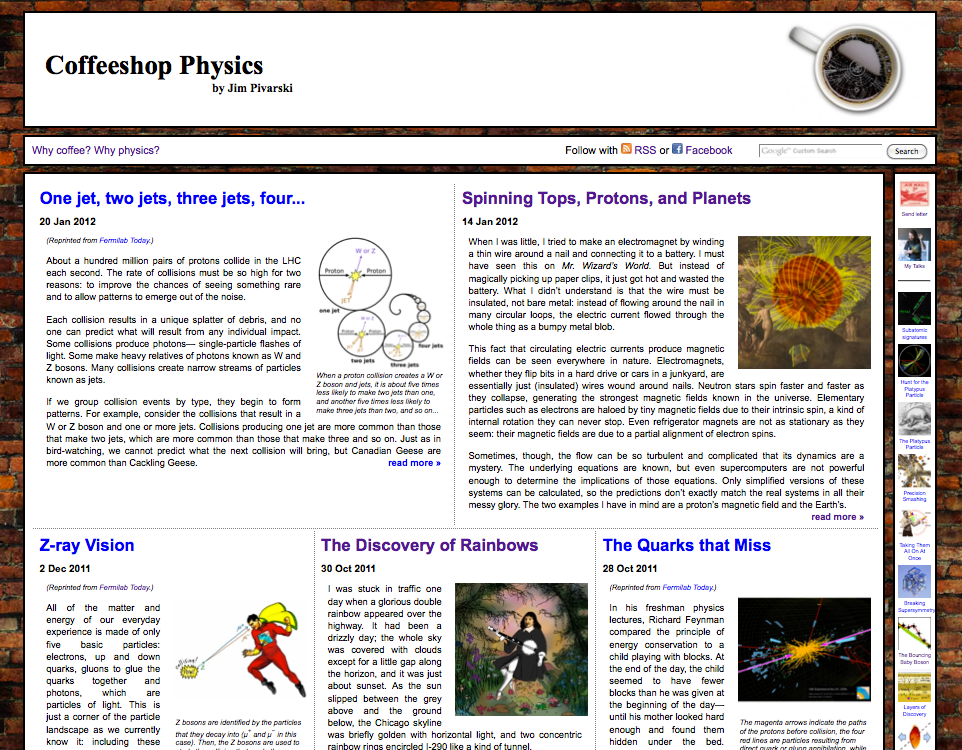
\includegraphics[width=0.75\linewidth]{coffeeshopphysics.png}
\end{center}
\end{frame}

\end{document}
